\documentclass[hidelinks, 12pt, oneside]{article}
\usepackage{graphicx}
\usepackage{bookmark}

\usepackage{epsfig}
\usepackage{epstopdf}

\usepackage{hyperref}
%\graphicspath{{}}
\begin{document}
 
%titlepage
\thispagestyle{empty}
\begin{center}
\begin{minipage}{0.75\linewidth}
    \centering
%University logo
   % 
\includegraphics[width=13cm]{graphics/universityLogo.jpg}
   % \rule{0\linewidth}{0.15\linewidth}\par

%Thesis title
    {\uppercase{\Large COS301: Mini Project Phase 1\par}}
   	{\uppercase{\Large Group 5 a \par}}
    \vspace{1cm}
%Author's name
    {\normalsize Khathutshelo Matidza 11072157\par}
    {\normalsize Renaldo van Dyk 12204359\par}
    {\normalsize Andreas du Preez 12207871\par}
    {\normalsize Sean Hill 12221458\par}
    {\normalsize Kgomotso Sito 12243273\par}
    {\normalsize Hlavutelo Maluleke 12318109\par}
    {\normalsize Siboniso Masilela 10416260\par}
    {\normalsize Semaka Malapane 13081129\par}
    
    \vspace{1cm}
    
    \hyperref[https://github.com/RenaldoV/COS301_Group5_a]{Github}\par
    \vspace{1cm}
	
\end{minipage}
\end{center}
\clearpage

\tableofcontents
\newpage

\section{User Management}
\subsection{Use case prioritization}
\subsubsection{Critical}
\begin{itemize}
  \item 1.1 updateAccountInformation
  \item 1.2 viewProfile
  \item 1.3 logIn
  \item 1.4 logOut
\end{itemize}

\subsubsection{Important}
\begin{itemize}
  \item 1.5 directMessage
\end{itemize}
\subsubsection{Nice-To-Have}


\subsection{Use case/Services contracts}
\subsubsection{Pre-Conditions}								%PRE CONDITIONS
\begin{itemize}
  \item 1.1 New information must be valid.
  \item 1.4 User must be logged in.
  \item 1.5a User must have a message.
  \item 1.5b User must have (a) valid recipient(s).
\end{itemize}

\subsubsection{Post-Conditions}%POST CONDITIONS	
\begin{itemize}
  \item 1.1 Information is updated on database.
  \item 1.4 User is logged out.
  \item 1.5 (The) recipient(s) recieve message.
\end{itemize}

\subsection{Required functionality} 
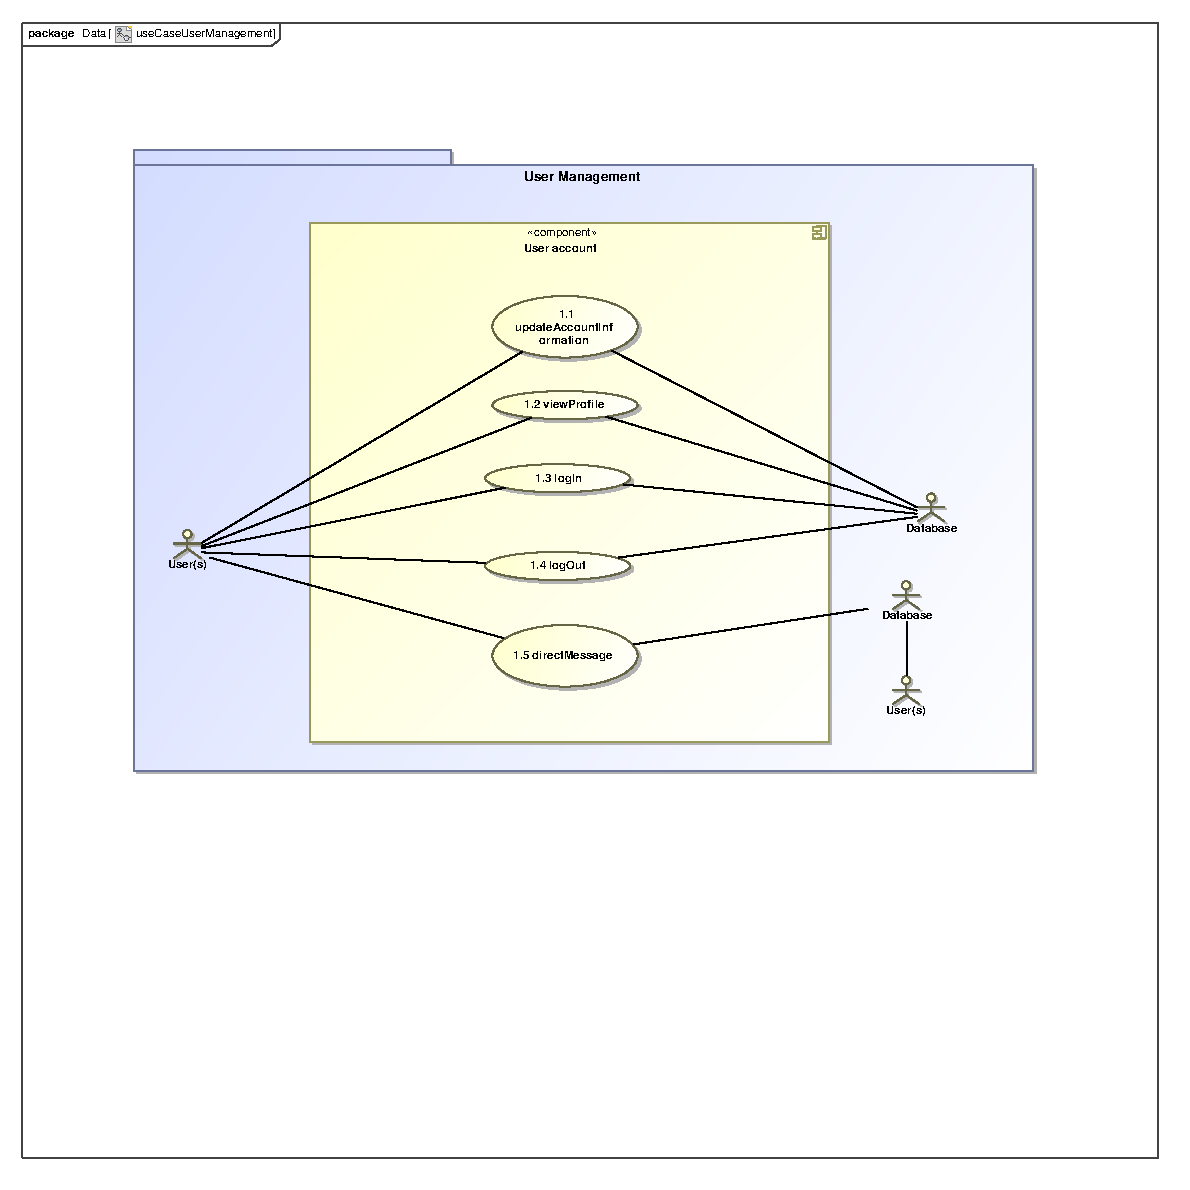
\includegraphics[scale=.9]{Sean/useCaseUserManagement.eps}\\

\subsection{Process specifications}
\subsubsection{User Management}
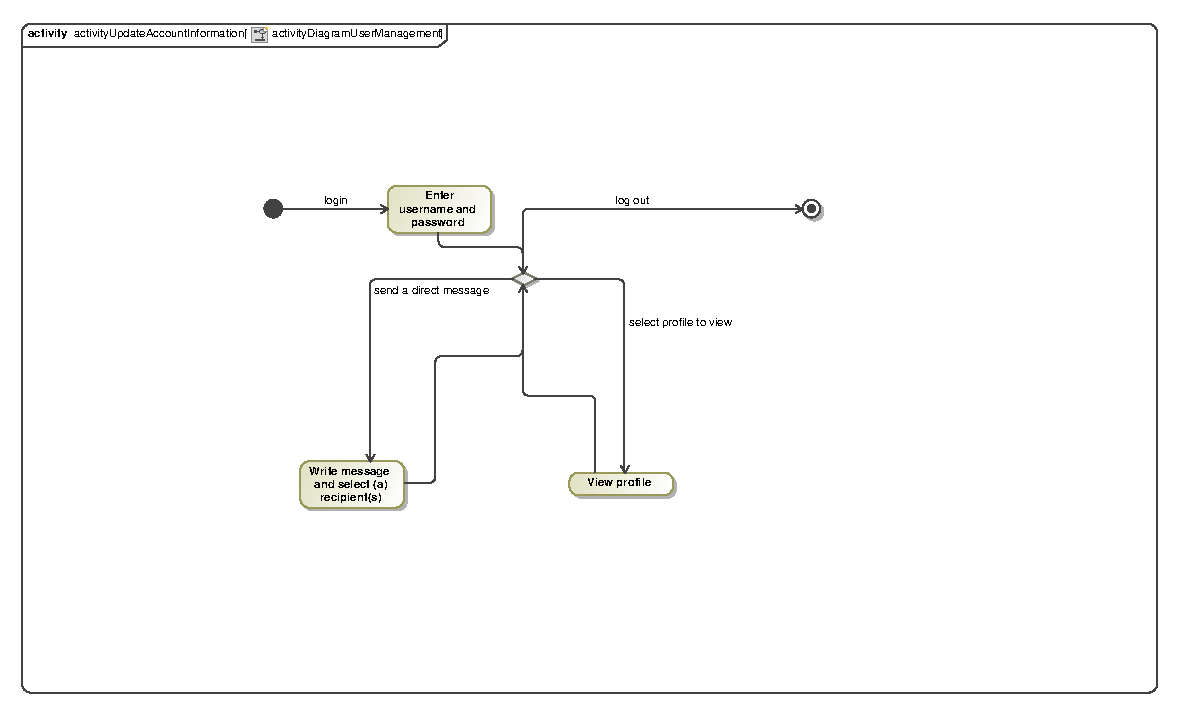
\includegraphics[scale=.9]{Sean/activityDiagramUserManagement.eps}\\

%Admin Management
\section{Admin Management}
\subsection{Use case prioritization}
\subsubsection{Critical}
\begin{itemize}
  \item 2.1 createAccount
  \item 2.2 deleteAccount
\end{itemize}
\subsubsection{Important}

\subsubsection{Nice-To-Have}
\begin{itemize}
  \item 2.3 customizeInterface
  \item 2.2 summarizeThreads
\end{itemize}
\subsubsection{Pre-Conditions}								%PRE CONDITIONS
\begin{itemize}
  \item 2.1 User must be a registered with the university
  \item 2.2 User must no longer be a student at the university
  \item 2.3 User must be of a specific status level(authority)
  \item 2.4 User must be of a specific status level(authority)
\end{itemize}

\subsubsection{Post-Conditions}%POST CONDITIONS	
\begin{itemize}
  \item 2.1 Account must exist
  \item 2.2 User account should be deleted along with all activities associated with it
  \item 2.3 Posts should be moved around and changes be visible
  \item 2.4 Summaries of threads should be created
\end{itemize}
\subsection{Required functionality} 
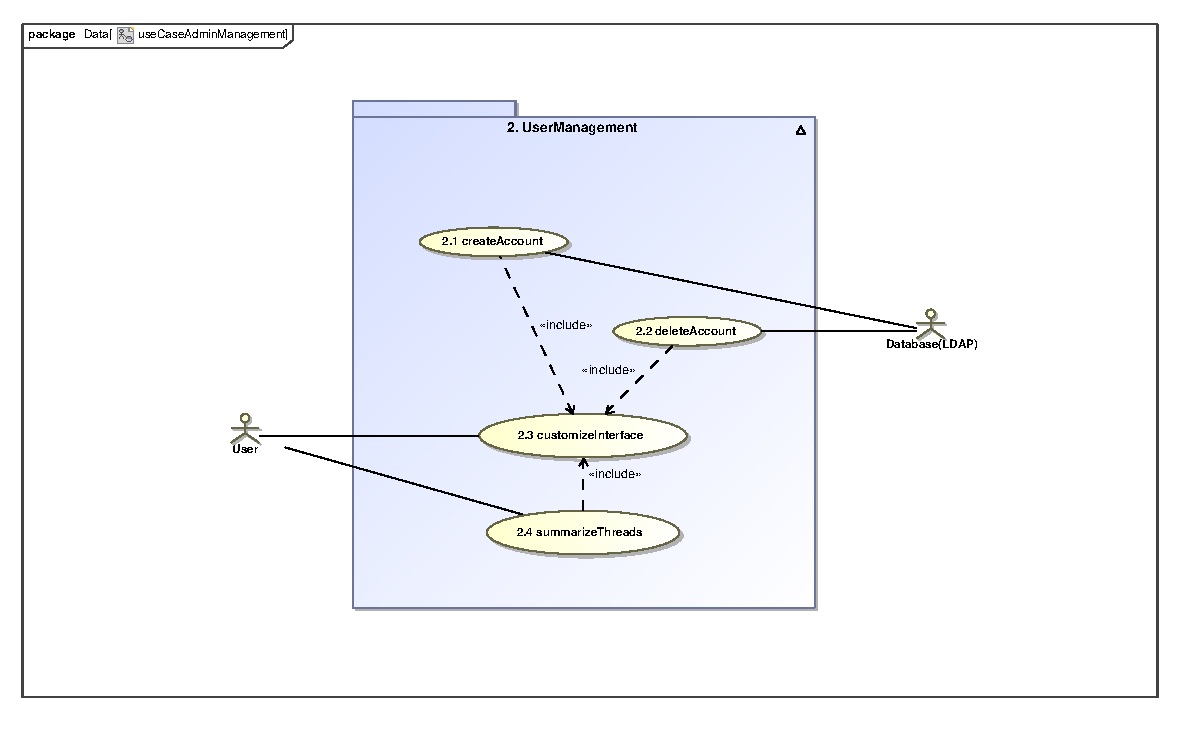
\includegraphics[scale=.9]{Shaun/graphics/useCaseAdminManagement.eps}\\

\subsection{Process specifications}
\subsubsection{User Management}
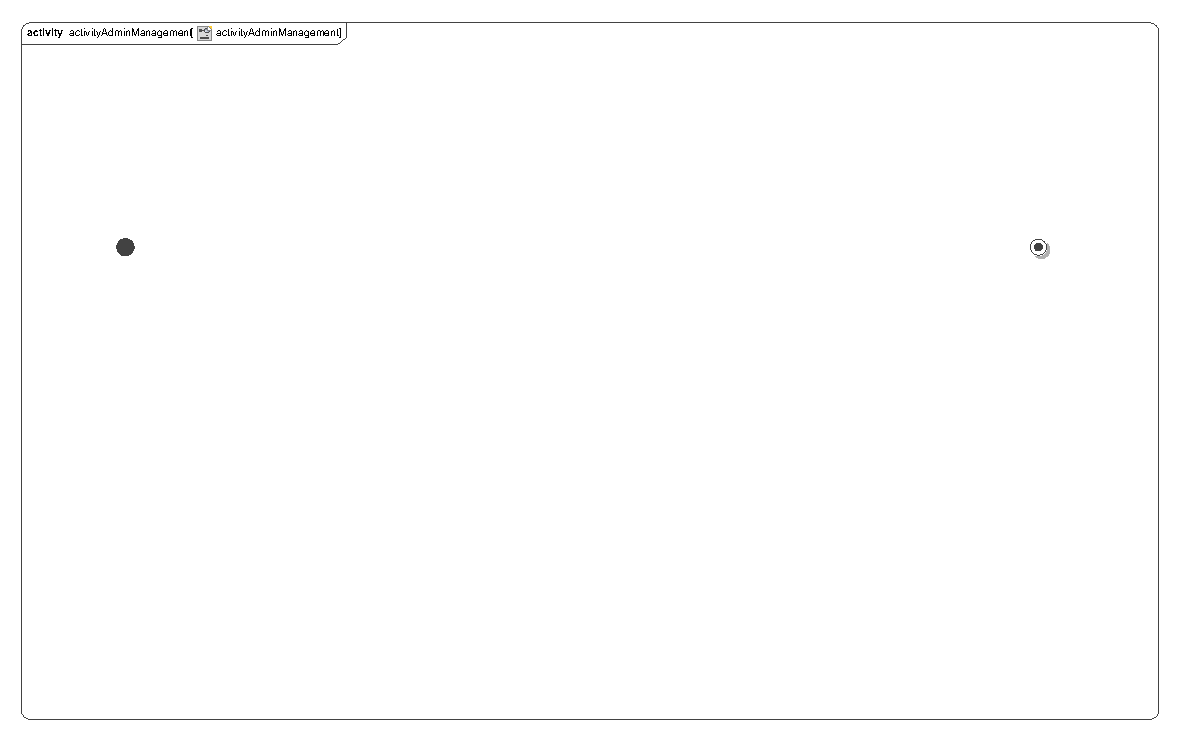
\includegraphics[scale=.9]{Shaun/graphics/activityAdminManagement.eps}\\


%Threads
\section{Threads}

\subsection{Use case prioritization}
\subsubsection{Critical}
\begin{itemize}
  \item 3.1 createRootThread
  \item 3.1.1 createSubThread
  \item 3.2 deleteThreads
  \item 3.2.1 archiveThreads
  \item 3.3 updateThreads
  \item 3.4 readThreads
\end{itemize}
\subsubsection{Important}
 \begin{itemize}
  \item 3.5 Read Tracking
 \end{itemize}

\subsection{Use case/Services contracts}
\subsubsection{Pre-Conditions}								%PRE CONDITIONS
\begin{itemize}
  \item 3.1 a) User must be logged into the system to create root threads
  \item 3.2 a) Thread must be read from database before it can be deleted
  \item 3.2.1 a) Thread must be deleted before it can be archived
  \item 3.3 a) User must be logged into the system to update the database
  \item     b) Before the database can be updated values must be changed
  \item 3.4 a) User must be logged into the system to read values from database
  \item 3.5 a) User must be logged into the system to see unread mesassages in bold
\end{itemize}

\subsubsection{Post-Conditions}								%POST CONDITIONS	
\begin{itemize}
\item 3.1 a) All threads will be visible to users who are logged into the system
\item     b) Threads will exist in database
\item 3.2 a) Threads will be acrhived.
\item     b) Threads will not be visible to users
\item 3.3 a) Updated threads will be visible
\item 3.5 a) Thread is marked as unread
\end{itemize}

\subsection{Required functionality} 
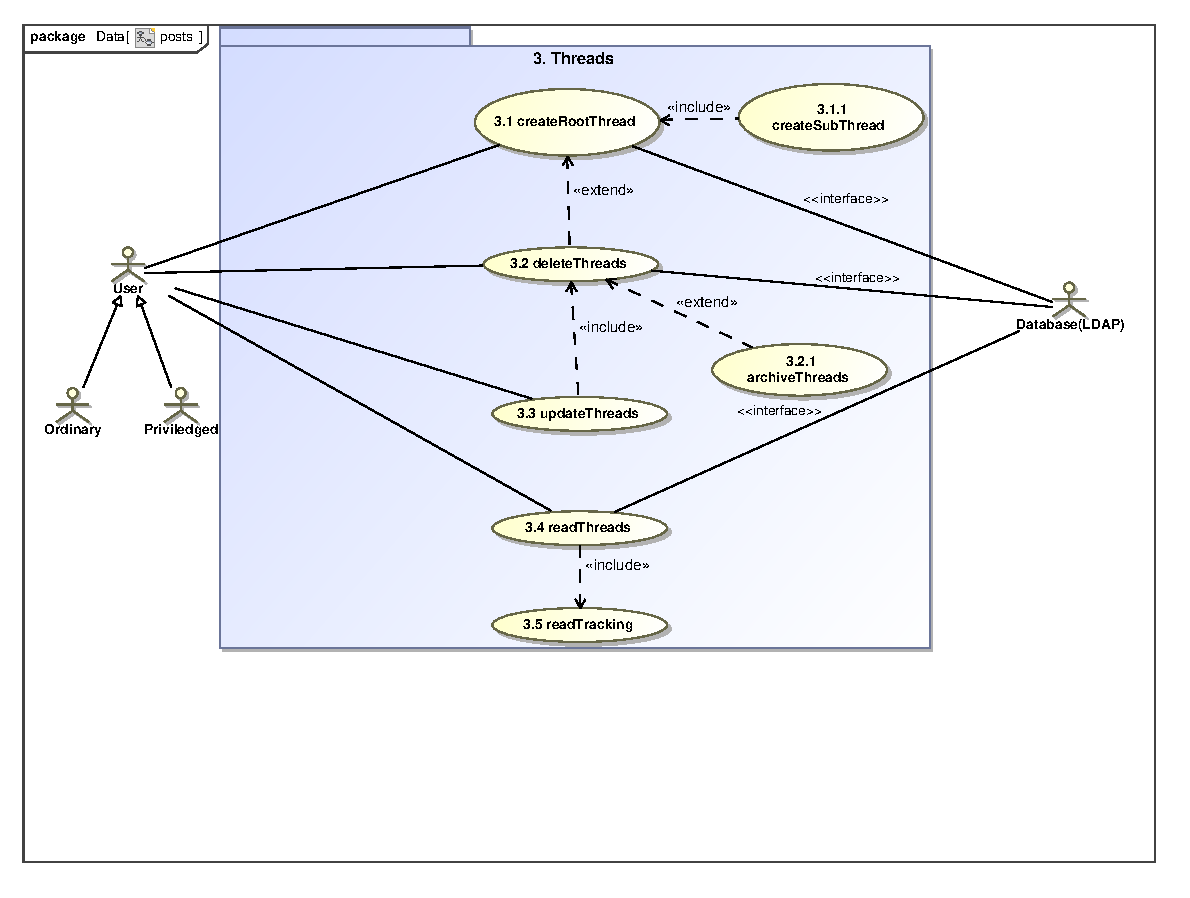
\includegraphics[scale=.9]{Renaldo/useCaseThreads.eps}\\

\subsection{Process specifications}
\subsubsection{Create Threads}
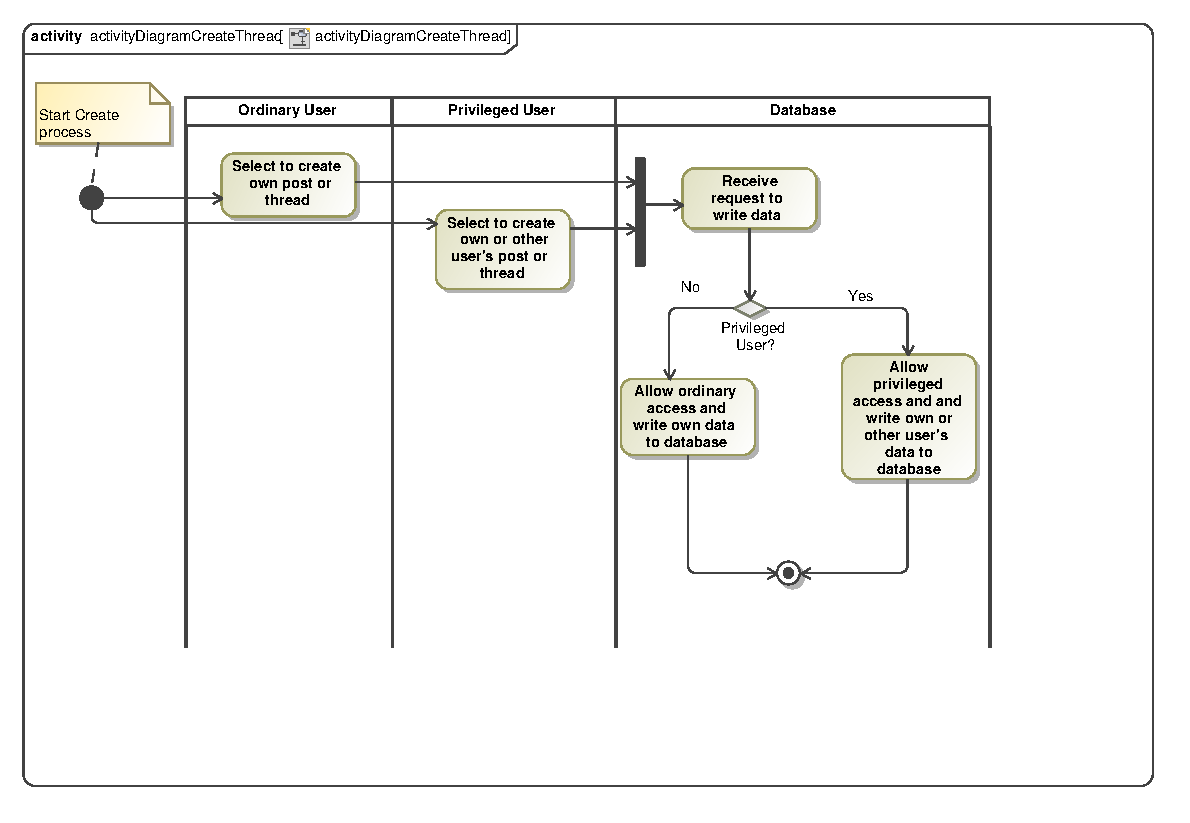
\includegraphics[scale=.9]{Renaldo/activityDiagramCreateThread.eps}\\

\subsubsection{Delete Threads}
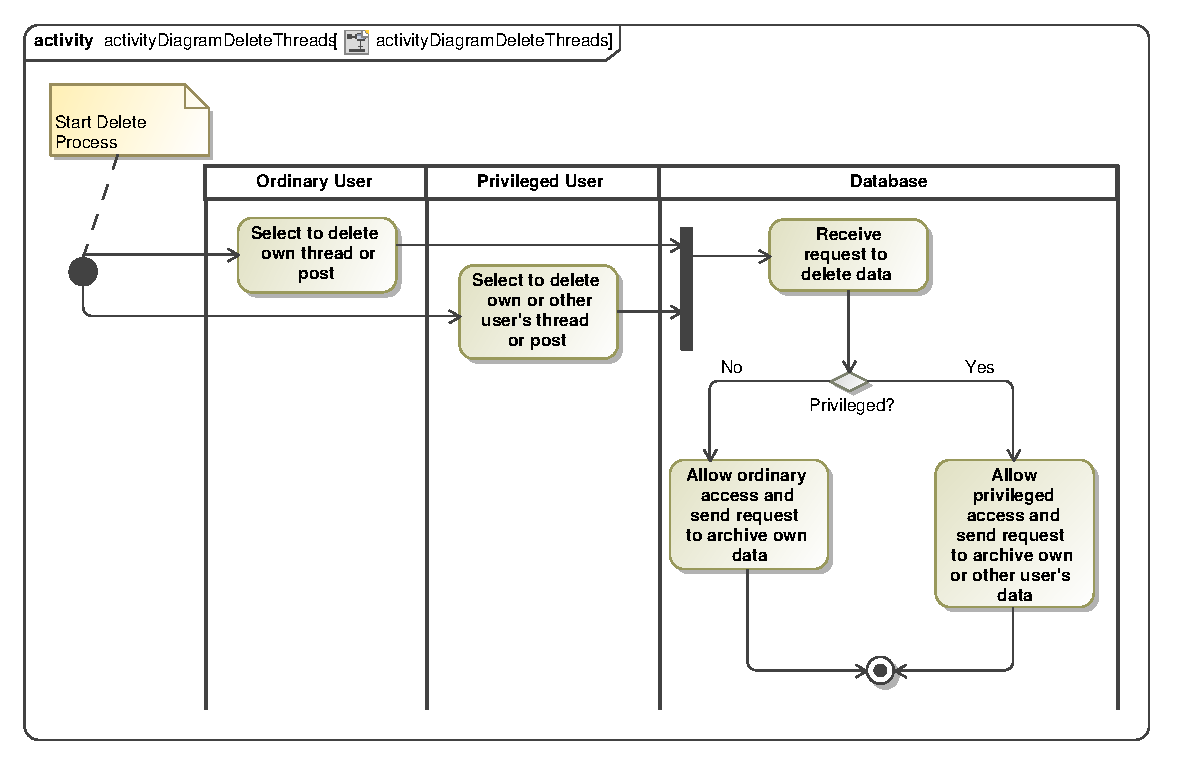
\includegraphics[scale=.9]{Renaldo/activityDiagramDeleteThreads.eps}\\

\subsubsection{Read Threads}
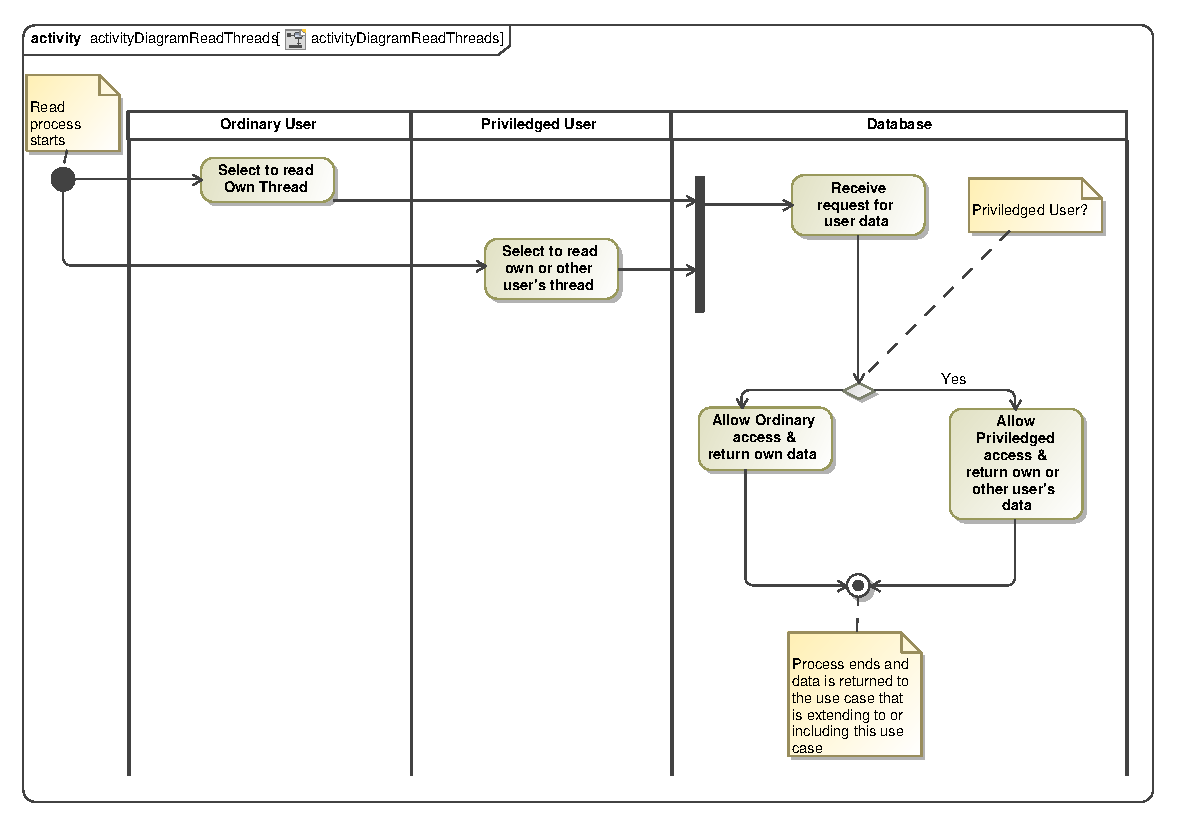
\includegraphics[scale=.9]{Andreas/activityDiagramReadThreads.eps}\\

\subsubsection{Read Tracking}
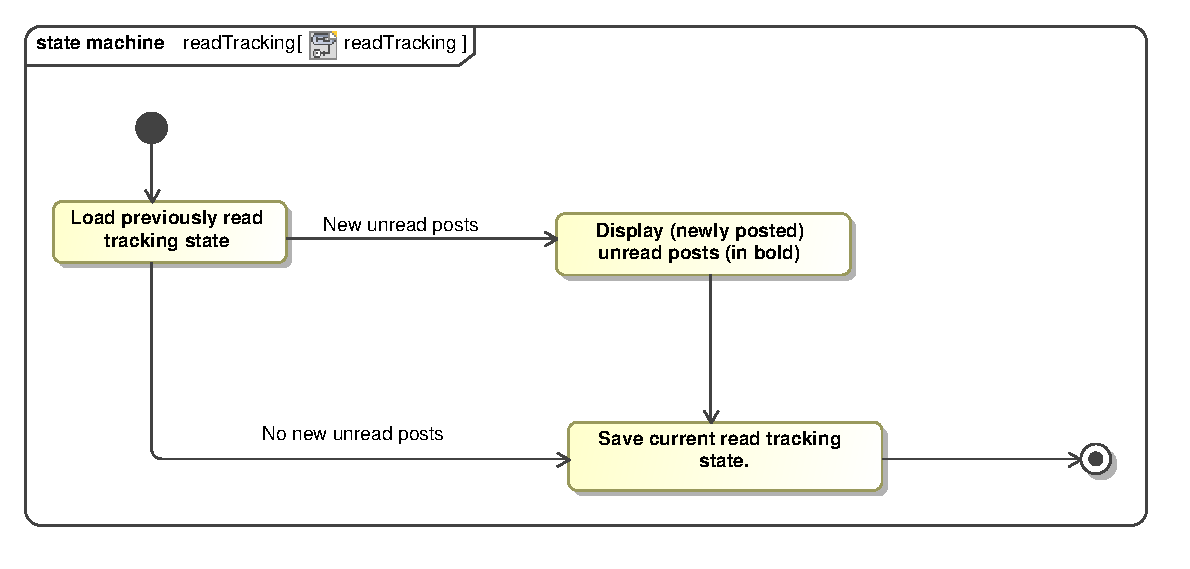
\includegraphics[scale=.9]{Andreas/stateDiagramreadTracking.eps}\\

\section{User Ranking}
\subsection{Use case prioritization}
\subsubsection{Critical}
\begin{itemize}
  \item 4.1 ratePost
  \item 4.3 manageUserRanking
\end{itemize}

\subsection{Important}
\begin{itemize}
  \item 4.2 markAllocation
\end{itemize}

\subsection{Use case/Services contracts}
\subsubsection{Pre-Conditions}								%PRE CONDITIONS
\begin{itemize}
 \item 4.1 Must be logged in
  \item 4.2 Must be logged in and also a lecturer or TA
  \item 4.3 Must be logged in and also a lecturer or TA
\end{itemize}

\subsubsection{Post-Conditions}%POST CONDITIONS	
\begin{itemize}
  \item 4.1 Post is rated
  \item 4.2 Student marks are allocated and status level changes accordingly
  \item 4.3 Students are ranked accordingly
\end{itemize}

\subsection{Required functionality} 
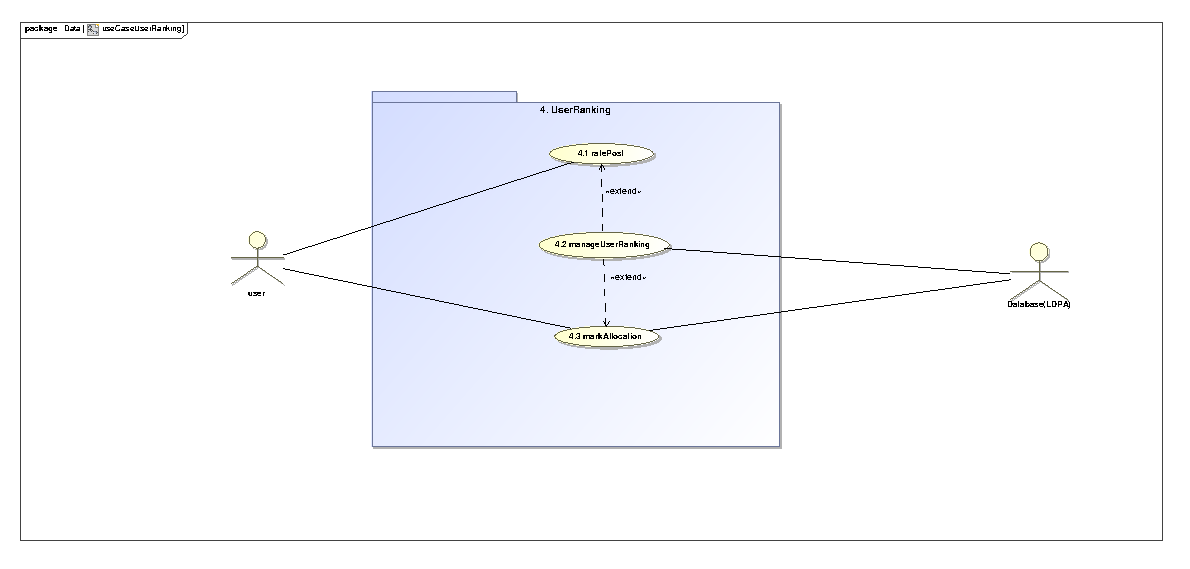
\includegraphics[scale=.9]{Kgomotso/graphics/useCaseUserRanking.eps}\\

\subsection{Process specifications}
\subsubsection{Rating Post}
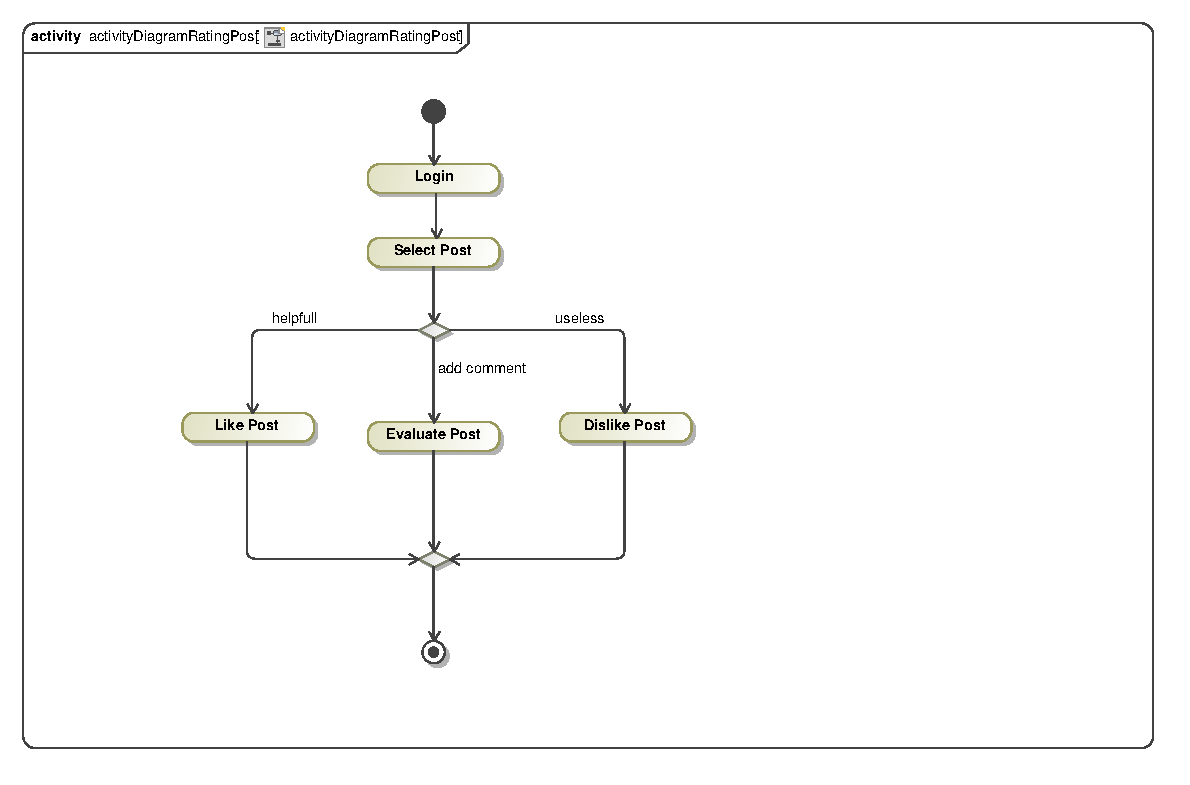
\includegraphics[scale=.9]{Kgomotso/graphics/activityDiagramRatingPost.eps}\\

\subsubsection{Mark Allocation}
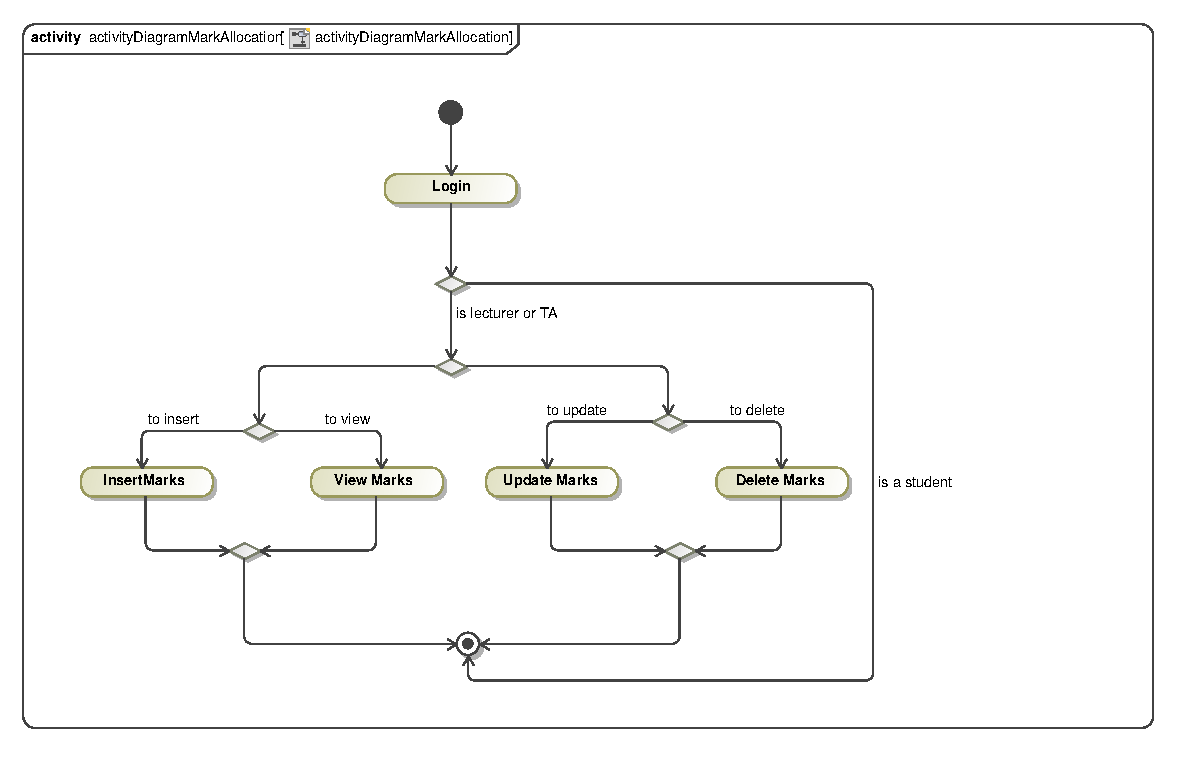
\includegraphics[scale=.9]{Kgomotso/graphics/activityDiagramMarkAllocation.eps}\\

\subsubsection{Manage Ranking}
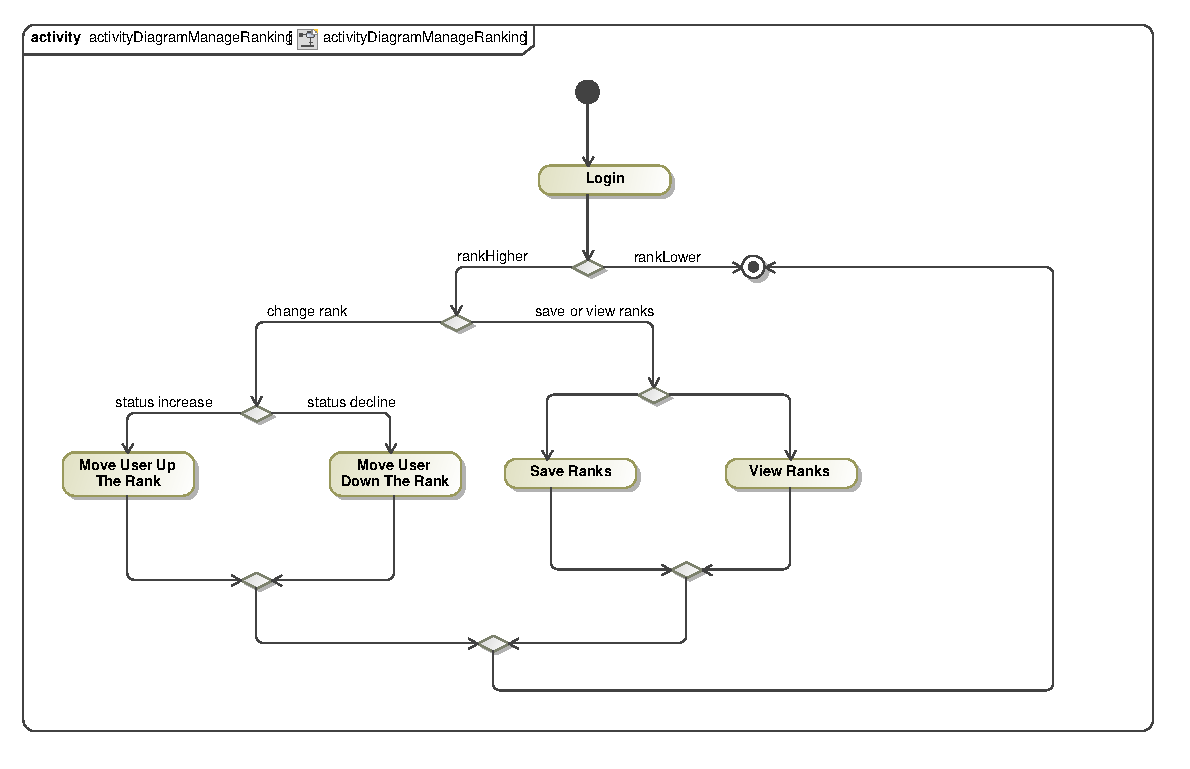
\includegraphics[scale=.9]{Kgomotso/graphics/activityDiagramManageRanking.eps}\\



\section{Social Tagging}
\subsection{Use case prioritization}
\subsubsection{Critical}
\begin{itemize}
  \item 5.1 createATtag
  \item 5.3 deleteTag
\end{itemize}

\subsubsection{Important}
\begin{itemize}
  \item 5.2 searchTag
  \item 5.4 updateTag
  \item 5.5 viewTag
\end{itemize}
\subsubsection{Nice-To-Have}
\begin{itemize}
  \item notify
\end{itemize}


\subsection{Use case/Services contracts}
\subsubsection{Pre-Conditions}								%PRE CONDITIONS
\begin{itemize}
  \item 5.1 User needs to be registered for the buzz space to be able to create tags
\end{itemize}

\subsubsection{Post-Conditions}%POST CONDITIONS	
\begin{itemize}
  \item 5.1 User should be able to access and or search for posts
\end{itemize}

\subsection{Request and Results Data Structures} 
\includegraphics[scale=.9]{Semaka/graphics/useCaseSocialTagging.eps}\\

\subsection{Process specifications}
\subsubsection{Social Tagging}
\includegraphics[scale=.9]{Semaka/graphics/activityDiagramSocialTagging.eps}\\
\section{Domain Model} 
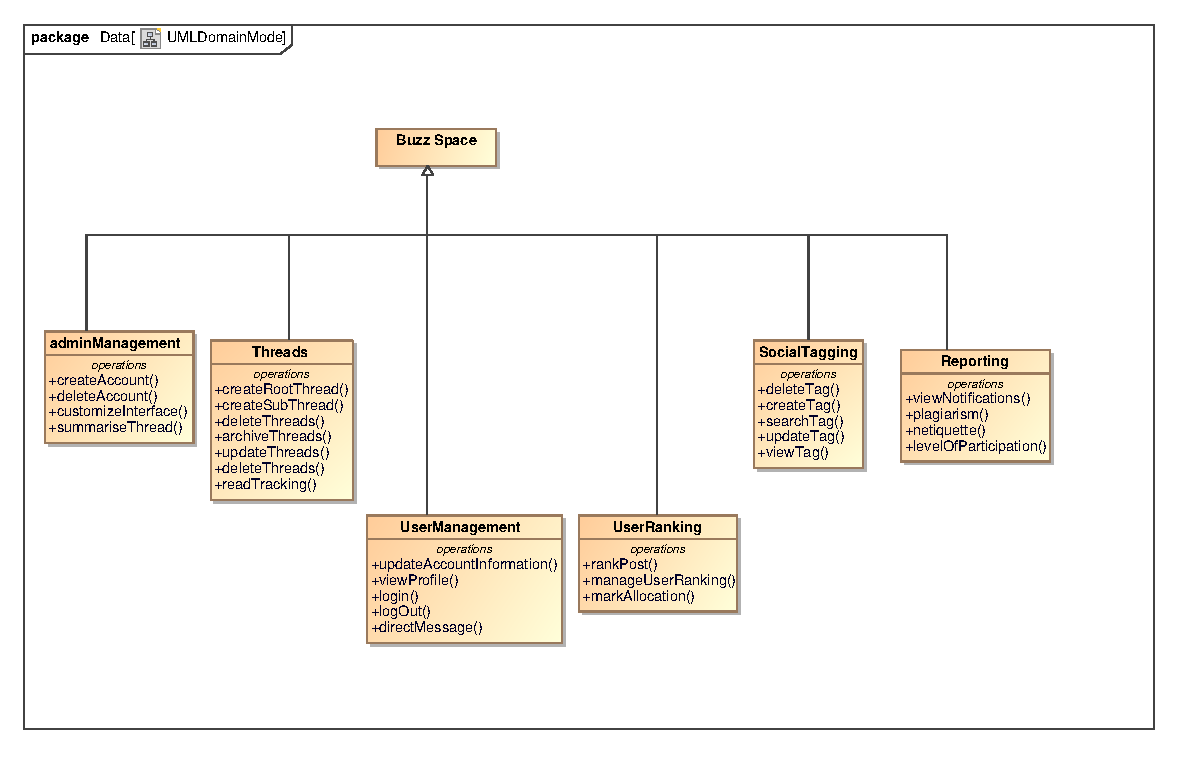
\includegraphics[scale=.9]{Kgomotso/graphics/UMLDomainModel.eps}\\

\end{document}
